% Options for packages loaded elsewhere
% Options for packages loaded elsewhere
\PassOptionsToPackage{unicode}{hyperref}
\PassOptionsToPackage{hyphens}{url}
\PassOptionsToPackage{dvipsnames,svgnames,x11names}{xcolor}
%
\documentclass[
]{article}
\usepackage{xcolor}
\usepackage{amsmath,amssymb}
\setcounter{secnumdepth}{5}
\usepackage{iftex}
\ifPDFTeX
  \usepackage[T1]{fontenc}
  \usepackage[utf8]{inputenc}
  \usepackage{textcomp} % provide euro and other symbols
\else % if luatex or xetex
  \usepackage{unicode-math} % this also loads fontspec
  \defaultfontfeatures{Scale=MatchLowercase}
  \defaultfontfeatures[\rmfamily]{Ligatures=TeX,Scale=1}
\fi
\usepackage{lmodern}
\ifPDFTeX\else
  % xetex/luatex font selection
\fi
% Use upquote if available, for straight quotes in verbatim environments
\IfFileExists{upquote.sty}{\usepackage{upquote}}{}
\IfFileExists{microtype.sty}{% use microtype if available
  \usepackage[]{microtype}
  \UseMicrotypeSet[protrusion]{basicmath} % disable protrusion for tt fonts
}{}
\makeatletter
\@ifundefined{KOMAClassName}{% if non-KOMA class
  \IfFileExists{parskip.sty}{%
    \usepackage{parskip}
  }{% else
    \setlength{\parindent}{0pt}
    \setlength{\parskip}{6pt plus 2pt minus 1pt}}
}{% if KOMA class
  \KOMAoptions{parskip=half}}
\makeatother
% Make \paragraph and \subparagraph free-standing
\makeatletter
\ifx\paragraph\undefined\else
  \let\oldparagraph\paragraph
  \renewcommand{\paragraph}{
    \@ifstar
      \xxxParagraphStar
      \xxxParagraphNoStar
  }
  \newcommand{\xxxParagraphStar}[1]{\oldparagraph*{#1}\mbox{}}
  \newcommand{\xxxParagraphNoStar}[1]{\oldparagraph{#1}\mbox{}}
\fi
\ifx\subparagraph\undefined\else
  \let\oldsubparagraph\subparagraph
  \renewcommand{\subparagraph}{
    \@ifstar
      \xxxSubParagraphStar
      \xxxSubParagraphNoStar
  }
  \newcommand{\xxxSubParagraphStar}[1]{\oldsubparagraph*{#1}\mbox{}}
  \newcommand{\xxxSubParagraphNoStar}[1]{\oldsubparagraph{#1}\mbox{}}
\fi
\makeatother


\usepackage{longtable,booktabs,array}
\usepackage{calc} % for calculating minipage widths
% Correct order of tables after \paragraph or \subparagraph
\usepackage{etoolbox}
\makeatletter
\patchcmd\longtable{\par}{\if@noskipsec\mbox{}\fi\par}{}{}
\makeatother
% Allow footnotes in longtable head/foot
\IfFileExists{footnotehyper.sty}{\usepackage{footnotehyper}}{\usepackage{footnote}}
\makesavenoteenv{longtable}
\usepackage{graphicx}
\makeatletter
\newsavebox\pandoc@box
\newcommand*\pandocbounded[1]{% scales image to fit in text height/width
  \sbox\pandoc@box{#1}%
  \Gscale@div\@tempa{\textheight}{\dimexpr\ht\pandoc@box+\dp\pandoc@box\relax}%
  \Gscale@div\@tempb{\linewidth}{\wd\pandoc@box}%
  \ifdim\@tempb\p@<\@tempa\p@\let\@tempa\@tempb\fi% select the smaller of both
  \ifdim\@tempa\p@<\p@\scalebox{\@tempa}{\usebox\pandoc@box}%
  \else\usebox{\pandoc@box}%
  \fi%
}
% Set default figure placement to htbp
\def\fps@figure{htbp}
\makeatother


% definitions for citeproc citations
\NewDocumentCommand\citeproctext{}{}
\NewDocumentCommand\citeproc{mm}{%
  \begingroup\def\citeproctext{#2}\cite{#1}\endgroup}
\makeatletter
 % allow citations to break across lines
 \let\@cite@ofmt\@firstofone
 % avoid brackets around text for \cite:
 \def\@biblabel#1{}
 \def\@cite#1#2{{#1\if@tempswa , #2\fi}}
\makeatother
\newlength{\cslhangindent}
\setlength{\cslhangindent}{1.5em}
\newlength{\csllabelwidth}
\setlength{\csllabelwidth}{3em}
\newenvironment{CSLReferences}[2] % #1 hanging-indent, #2 entry-spacing
 {\begin{list}{}{%
  \setlength{\itemindent}{0pt}
  \setlength{\leftmargin}{0pt}
  \setlength{\parsep}{0pt}
  % turn on hanging indent if param 1 is 1
  \ifodd #1
   \setlength{\leftmargin}{\cslhangindent}
   \setlength{\itemindent}{-1\cslhangindent}
  \fi
  % set entry spacing
  \setlength{\itemsep}{#2\baselineskip}}}
 {\end{list}}
\usepackage{calc}
\newcommand{\CSLBlock}[1]{\hfill\break\parbox[t]{\linewidth}{\strut\ignorespaces#1\strut}}
\newcommand{\CSLLeftMargin}[1]{\parbox[t]{\csllabelwidth}{\strut#1\strut}}
\newcommand{\CSLRightInline}[1]{\parbox[t]{\linewidth - \csllabelwidth}{\strut#1\strut}}
\newcommand{\CSLIndent}[1]{\hspace{\cslhangindent}#1}



\setlength{\emergencystretch}{3em} % prevent overfull lines

\providecommand{\tightlist}{%
  \setlength{\itemsep}{0pt}\setlength{\parskip}{0pt}}



 


\makeatletter
\@ifpackageloaded{caption}{}{\usepackage{caption}}
\AtBeginDocument{%
\ifdefined\contentsname
  \renewcommand*\contentsname{Table of contents}
\else
  \newcommand\contentsname{Table of contents}
\fi
\ifdefined\listfigurename
  \renewcommand*\listfigurename{List of Figures}
\else
  \newcommand\listfigurename{List of Figures}
\fi
\ifdefined\listtablename
  \renewcommand*\listtablename{List of Tables}
\else
  \newcommand\listtablename{List of Tables}
\fi
\ifdefined\figurename
  \renewcommand*\figurename{Figure}
\else
  \newcommand\figurename{Figure}
\fi
\ifdefined\tablename
  \renewcommand*\tablename{Table}
\else
  \newcommand\tablename{Table}
\fi
}
\@ifpackageloaded{float}{}{\usepackage{float}}
\floatstyle{ruled}
\@ifundefined{c@chapter}{\newfloat{codelisting}{h}{lop}}{\newfloat{codelisting}{h}{lop}[chapter]}
\floatname{codelisting}{Listing}
\newcommand*\listoflistings{\listof{codelisting}{List of Listings}}
\makeatother
\makeatletter
\makeatother
\makeatletter
\@ifpackageloaded{caption}{}{\usepackage{caption}}
\@ifpackageloaded{subcaption}{}{\usepackage{subcaption}}
\makeatother
\usepackage{bookmark}
\IfFileExists{xurl.sty}{\usepackage{xurl}}{} % add URL line breaks if available
\urlstyle{same}
\hypersetup{
  pdftitle={Finding the mjor descriptors of species networks},
  pdfauthor={Tanya Strydom; Andrew P. Beckerman},
  pdfkeywords={food web, structure, dimensionality reduction},
  colorlinks=true,
  linkcolor={blue},
  filecolor={Maroon},
  citecolor={Blue},
  urlcolor={Blue},
  pdfcreator={LaTeX via pandoc}}



\title{Finding the mjor descriptors of species networks}
\author{Tanya Strydom %
%
\textsuperscript{%
%
1%
}%
; Andrew P. Beckerman %
%
\textsuperscript{%
%
1%
}%
}
\date{2025-06-02}

\usepackage{setspace}
\usepackage[left]{lineno}
\usepackage[letterpaper]{geometry}

\usepackage[nolists,noheads,markers]{endfloat}
\geometry{margin=2.5cm}

\begin{document}

\thispagestyle{empty}
{\bfseries\sffamily\Large Finding the mjor descriptors of species
networks}
\vfil
Tanya Strydom %
%
\textsuperscript{%
%
1%
}%
; Andrew P. Beckerman %
%
\textsuperscript{%
%
1%
}%

\vfil
{\small
\textbf{Abstract:} TODO
\vfil
\textbf{Keywords:} %
food web, structure, %
dimensionality reduction%
}
\clearpage
\setcounter{page}{1}
\doublespacing
\linenumbers


Blah blah blah Vermaat et al. (2009)

\emph{``It is incumbent on network ecologists to establish clearly the
independence and uniqueness of the descriptive metrics used.''} - Lau et
al. (2017)

\begin{longtable}[]{@{}
  >{\raggedright\arraybackslash}p{(\linewidth - 6\tabcolsep) * \real{0.2254}}
  >{\raggedright\arraybackslash}p{(\linewidth - 6\tabcolsep) * \real{0.3239}}
  >{\raggedright\arraybackslash}p{(\linewidth - 6\tabcolsep) * \real{0.2254}}
  >{\raggedright\arraybackslash}p{(\linewidth - 6\tabcolsep) * \real{0.2254}}@{}}
\caption{An informative caption about the different network
properties}\label{tbl-properties}\tabularnewline
\toprule\noalign{}
\begin{minipage}[b]{\linewidth}\raggedright
Label
\end{minipage} & \begin{minipage}[b]{\linewidth}\raggedright
Definition
\end{minipage} & \begin{minipage}[b]{\linewidth}\raggedright
``Function''
\end{minipage} & \begin{minipage}[b]{\linewidth}\raggedright
Reference (for maths), can make footnotes probs
\end{minipage} \\
\midrule\noalign{}
\endfirsthead
\toprule\noalign{}
\begin{minipage}[b]{\linewidth}\raggedright
Label
\end{minipage} & \begin{minipage}[b]{\linewidth}\raggedright
Definition
\end{minipage} & \begin{minipage}[b]{\linewidth}\raggedright
``Function''
\end{minipage} & \begin{minipage}[b]{\linewidth}\raggedright
Reference (for maths), can make footnotes probs
\end{minipage} \\
\midrule\noalign{}
\endhead
\bottomrule\noalign{}
\endlastfoot
Basal & Percentage of basal taxa, defined as species who have a
vulnerability of zero & & \\
Connectance & \(L/S^2\), where \(S\) is the number of species and \(L\)
the number of links & & \\
Cannibal & Percentage of species that are cannibals & & \\
ChLen & Mean food chain length, averaged over all species (where a food
chain is defined as a continuous path from a `basal' to a `top' species)
& & \\
ChSD & Standard deviation of ChLen & & \\
ChNum & log number of food chains & & \\
Clust & mean clustering coefficient (probability that two taxa linked to
the same taxon are also linked) & & \textbf{TODO} \\
GenSD & Normalized standard deviation of generality of a species
standardized by \(L/S\) & & Williams \& Martinez (2008) \\
Herbivore & Percentage of herbivores plus detritivores (taxa that feed
only on basal taxa) & & \\
Intermediate & Percentage of intermediate taxa (with both consumers and
resources) & & \\
LinkSD & Normalized standard deviation of links (number of consumers
plus resources per taxon) & & \\
Loop & Percentage of taxa in loops (food chains in which a taxon occurs
twice) & & \\
L/S & links per species & & \\
MaxSim & Mean of the maximum trophic similarity of each taxon to other
taxa, the number of predators and prey shared by a pair of species
divided by their total number of predators and prey & & \textbf{TODO} \\
Omnivory & Percentage of omnivores (taxa that feed on \(\geq\) 2 taxa
with different trophic levels) & & \\
Path & characteristic path length, the mean shortest food chain length
between species pairs & & \\
Richness & Number of nodes in the network & & \\
TL & Prey-weighted trophic level averaged across taxa & & Williams \&
Martinez (2004) \\
Top & Percentage of top taxa (taxa without consumers) & & \\
VulSD & Normalized standard deviation of vulnerability of a species
standardized by \(L/S\) & & \\
Links & The number of links in the network & & \\
Diameter & Diameter can also be measured as the average of the distances
between each pair of nodes in the network & & Delmas et al. (2019) \\
\(\rho\) & Spectral radius is a a conceptual analog to nestedness (and
more appropriate for unipartite networks). It is defined as the absolute
value of the largest real part of the eigenvalues of the
\emph{undirected} adjacency matrix & & Staniczenko et al. (2013) \\
Complexity & SVD complexity of a network, defined as the Pielou entropy
of its singular values & Something about structural v behavioural
complexity being captured & Strydom et al. (2021) \\
Centrality & Centrality is a measure of how `influential' a species is,
under various definitions of `influence'\ldots{} & Centrality can help
in quantifying the importance of species in a network & \\
S1 & Number of linear chains & & Stouffer et al. (2007) Milo et al.
(2002) \\
S2 & Number of omnivory motifs & & Stouffer et al. (2007) Milo et al.
(2002) \\
S4 & Number of apparent competition motifs & & Stouffer et al. (2007)
Milo et al. (2002) \\
S5 & Number of direct competition motifs & & Stouffer et al. (2007) Milo
et al. (2002) \\
Intervality & & & \textbf{TODO} Stouffer et al. (2006) \\
\end{longtable}

\begin{longtable}[]{@{}lllr@{}}

\caption{\label{tbl-corr}Here is a table showing the correlation of the
different network properties with the first three dimensions of the PCA}

\tabularnewline

\toprule\noalign{}
Property & PCA 1 (27\%) & PCA 2 (24\%) & PCA 3 (11\%) \\
\midrule\noalign{}
\endhead
\bottomrule\noalign{}
\endlastfoot
richness & \textbf{0.8} & 0.46 & -0.11 \\
links & \textbf{0.89} & 0.14 & -0.16 \\
connectance & 0.05 & -0.9 & 0.02 \\
diameter & \textbf{0.81} & -0.06 & 0.14 \\
complexity & -0.28 & 0.48 & 0.41 \\
distance & 0.41 & 0.13 & -0.03 \\
basal & -0.29 & 0.38 & -0.73 \\
top & -0.24 & 0.59 & 0.55 \\
intermediate & 0.4 & -0.68 & 0.32 \\
herbivory & -0.29 & 0.51 & 0.13 \\
omnivory & 0.52 & -0.71 & 0.18 \\
cannibal & 0.29 & -0.72 & -0.19 \\
l\_S & \textbf{0.78} & -0.33 & -0.18 \\
GenSD & -0.1 & 0.42 & -0.80 \\
VulSD & -0.05 & \textbf{0.76} & 0.31 \\
TL & 0.59 & -0.13 & 0.39 \\
ChLen & 0.17 & 0.45 & 0.30 \\
ChSD & 0.42 & 0.05 & 0.15 \\
ChNum & 0.19 & \textbf{0.69} & 0.42 \\
path & 0.66 & 0.09 & 0.17 \\
LinkSD & 0.04 & 0.63 & -0.54 \\
S1 & \textbf{0.82} & 0.29 & 0.00 \\
S2 & \textbf{0.84} & 0.12 & -0.06 \\
S4 & \textbf{0.74} & 0.43 & -0.13 \\
S5 & \textbf{0.76} & 0.39 & -0.22 \\
ρ & 0.14 & -0.82 & -0.24 \\
centrality & -0.49 & -0.29 & 0.21 \\
loops & 0.45 & 0.12 & 0.07 \\

\end{longtable}

\textsubscript{Source:
\href{https://BecksLab.github.io/ms_feature_selection/index.qmd.html}{Article
Notebook}}

\begin{figure}[H]

{\centering \pandocbounded{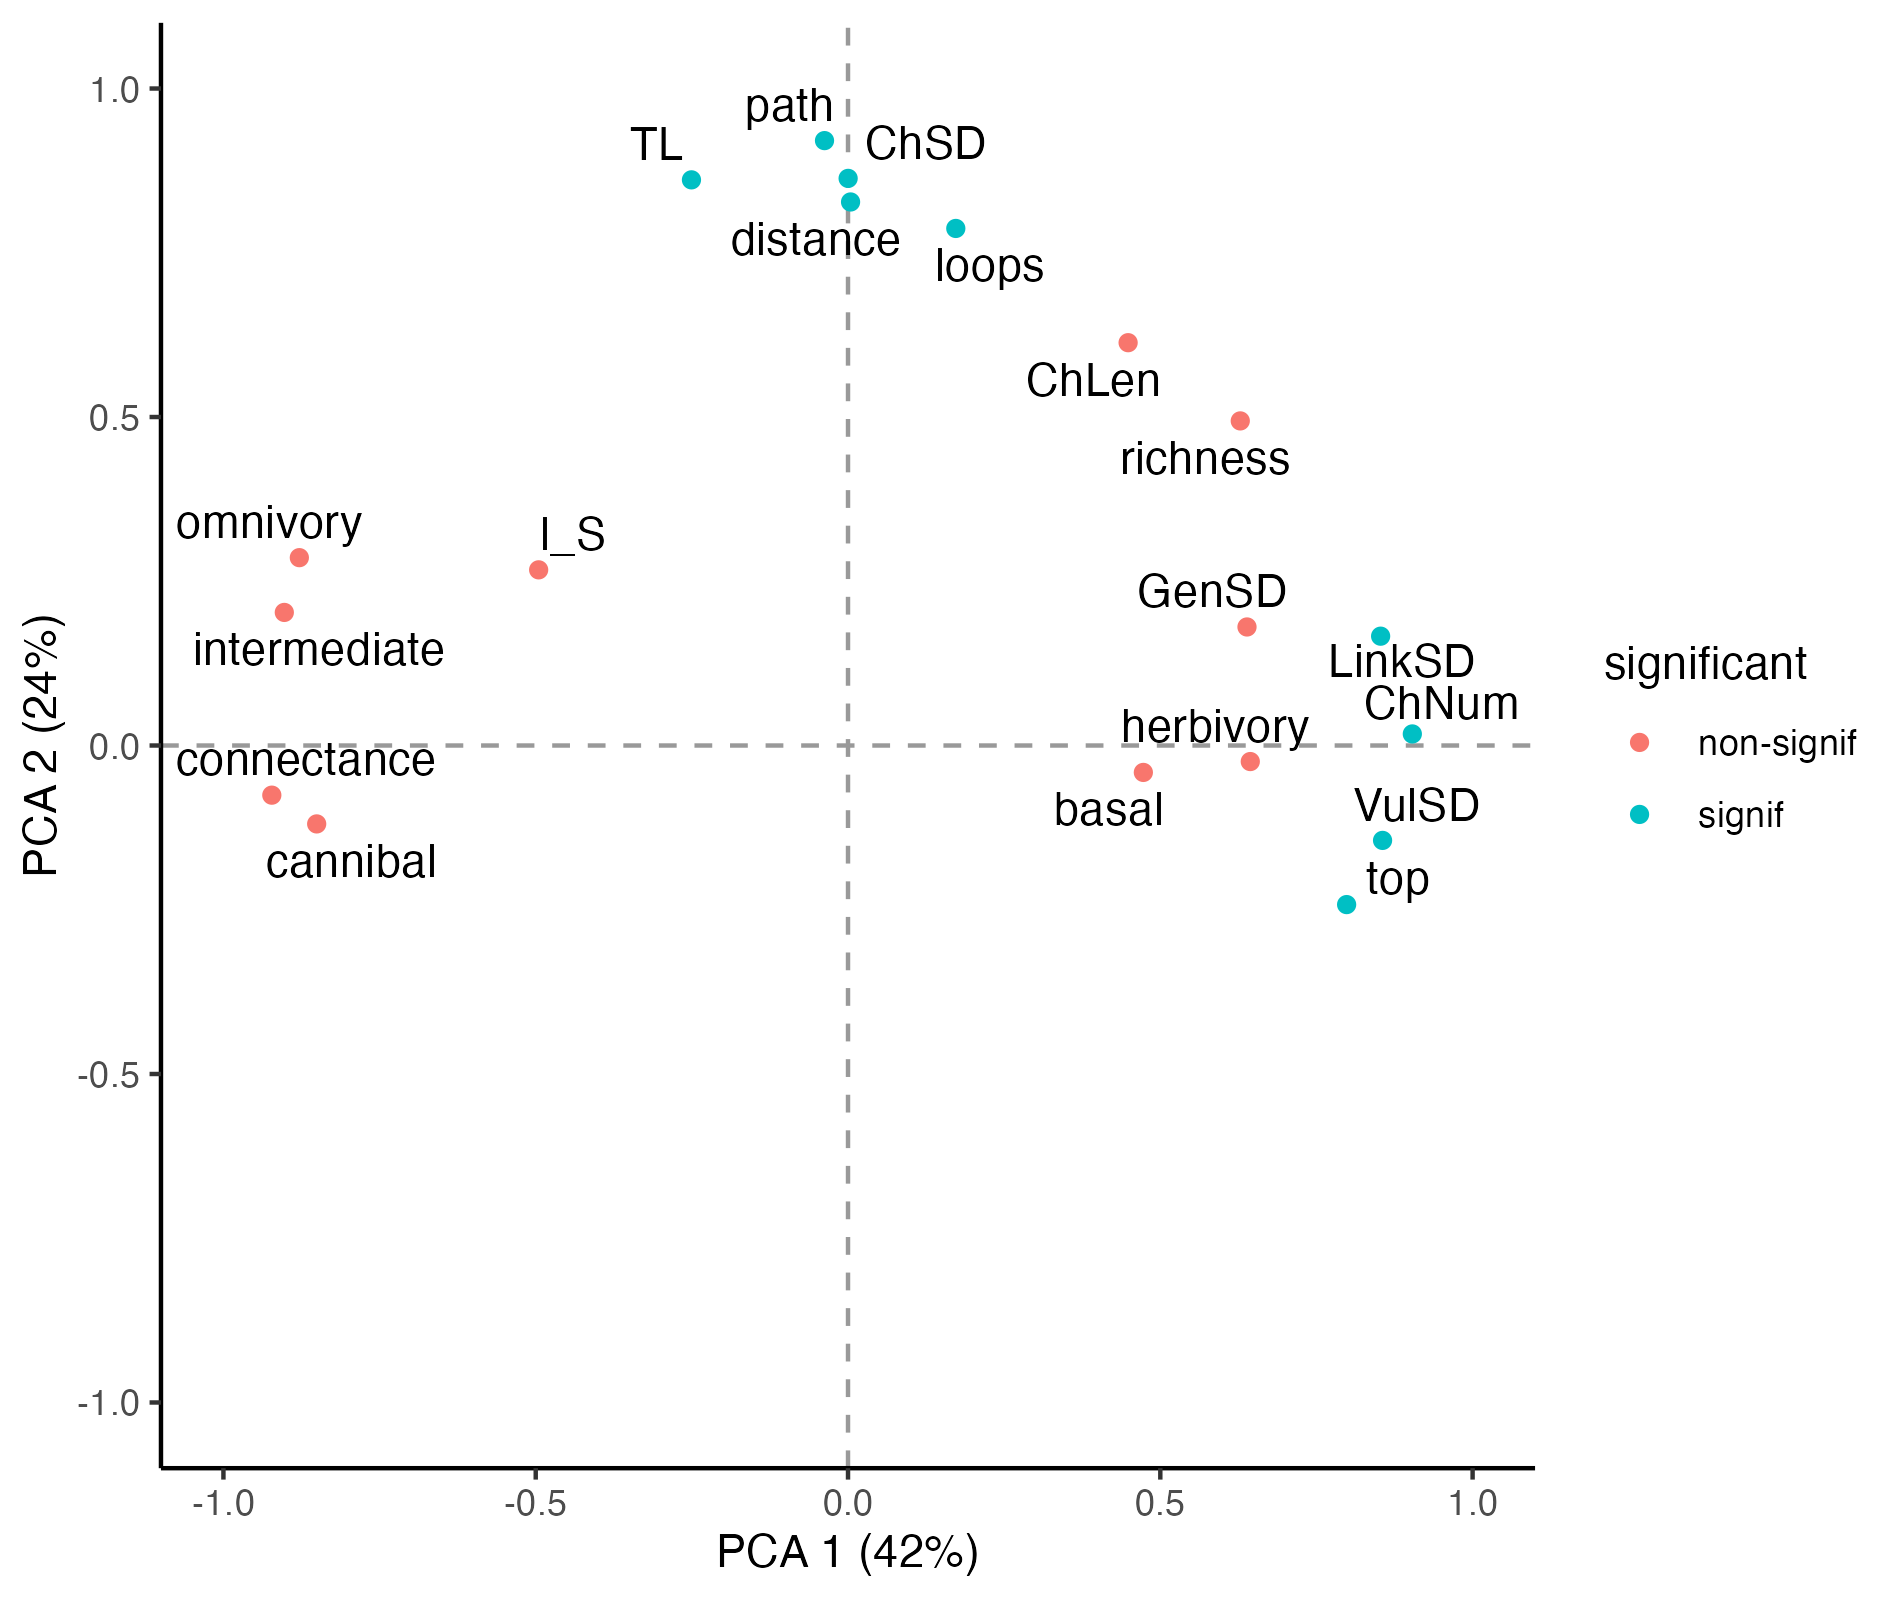
\includegraphics[keepaspectratio]{figures/pca_vermaat.png}}

}

\caption{VERMAAT networks only}

\end{figure}%

\begin{figure}[H]

{\centering \pandocbounded{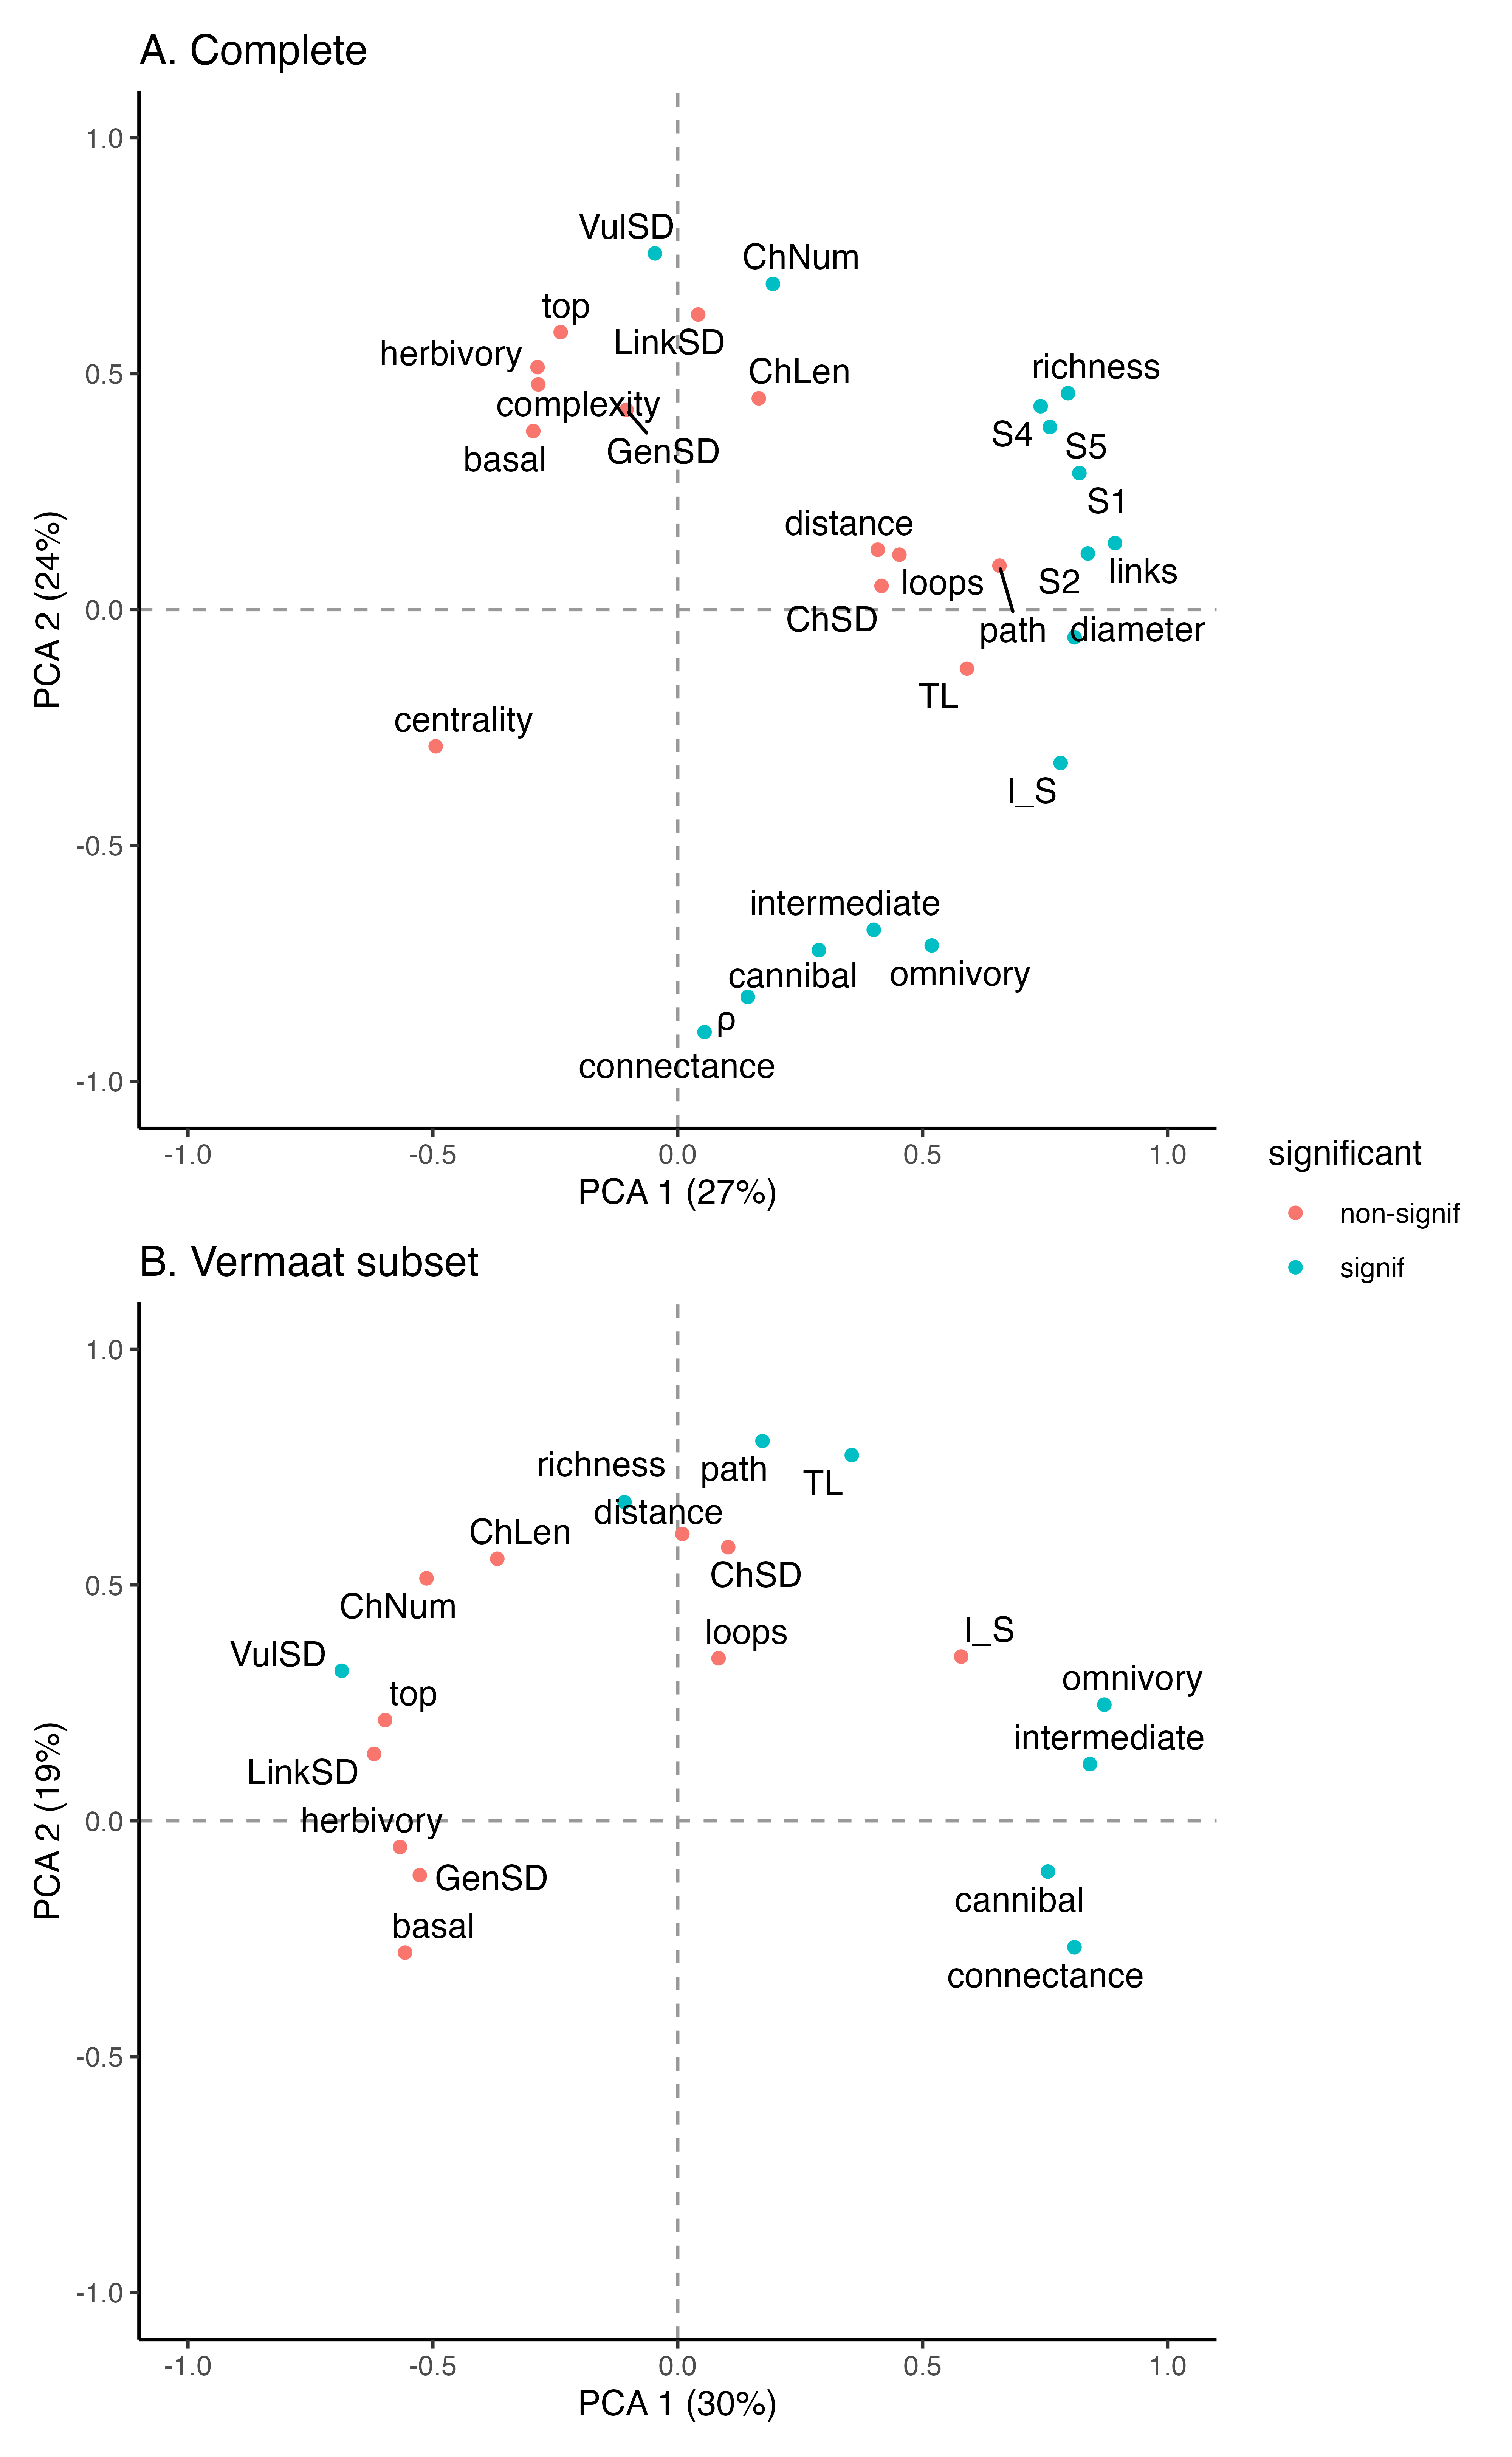
\includegraphics[keepaspectratio]{figures/pca_allNetworks.png}}

}

\caption{All networks. Vermaat subset = using only the structural
measures from Vermaat}

\end{figure}%

\section*{References}\label{references}
\addcontentsline{toc}{section}{References}

\phantomsection\label{refs}
\begin{CSLReferences}{1}{0}
\bibitem[\citeproctext]{ref-delmasAnalysingEcologicalNetworks2019}
Delmas, E., Besson, M., Brice, M.-H., Burkle, L. A., Riva, G. V. D.,
Fortin, M.-J., Gravel, D., Guimarães, P. R., Hembry, D. H., Newman, E.
A., Olesen, J. M., Pires, M. M., Yeakel, J. D., \& Poisot, T. (2019).
Analysing ecological networks of species interactions. \emph{Biological
Reviews}, \emph{94}(1), 16--36. \url{https://doi.org/10.1111/brv.12433}

\bibitem[\citeproctext]{ref-lauEcologicalNetworkMetrics2017}
Lau, M. K., Borrett, S. R., Baiser, B., Gotelli, N. J., \& Ellison, A.
M. (2017). Ecological network metrics: Opportunities for synthesis.
\emph{Ecosphere}, \emph{8}(8), e01900.
\url{https://doi.org/10.1002/ecs2.1900}

\bibitem[\citeproctext]{ref-miloNetworkMotifsSimple2002}
Milo, R., Shen-Orr, S., Itzkovitz, S., Kashtan, N., Chklovskii, D., \&
Alon, U. (2002). Network {Motifs}: {Simple Building Blocks} of {Complex
Networks}. \emph{Science}, \emph{298}(5594), 824--827.
\url{https://doi.org/10.1126/science.298.5594.824}

\bibitem[\citeproctext]{ref-staniczenkoGhostNestednessEcological2013}
Staniczenko, P. P. A., Kopp, J. C., \& Allesina, S. (2013). The ghost of
nestedness in ecological networks. \emph{Nature Communications},
\emph{4}(1), 1391. \url{https://doi.org/10.1038/ncomms2422}

\bibitem[\citeproctext]{ref-stoufferRobustMeasureFood2006a}
Stouffer, D. B., Camacho, J., \& Amaral, L. A. N. (2006). A robust
measure of food web intervality. \emph{Proceedings of the National
Academy of Sciences}, \emph{103}(50), 19015--19020.
\url{https://doi.org/10.1073/pnas.0603844103}

\bibitem[\citeproctext]{ref-stoufferEvidenceExistenceRobust2007}
Stouffer, D. B., Camacho, J., Jiang, W., \& Nunes Amaral, L. A. (2007).
Evidence for the existence of a robust pattern of prey selection in food
webs. \emph{Proceedings of the Royal Society B: Biological Sciences},
\emph{274}(1621), 1931--1940.
\url{https://doi.org/10.1098/rspb.2007.0571}

\bibitem[\citeproctext]{ref-strydomSVDEntropyReveals2021}
Strydom, T., Dalla Riva, G. V., \& Poisot, T. (2021). {SVD Entropy
Reveals} the {High Complexity} of {Ecological Networks}. \emph{Frontiers
in Ecology and Evolution}, \emph{9}.
\url{https://doi.org/10.3389/fevo.2021.623141}

\bibitem[\citeproctext]{ref-vermaatMajorDimensionsFoodweb2009}
Vermaat, J. E., Dunne, J. A., \& Gilbert, A. J. (2009). Major dimensions
in food-web structure properties. \emph{Ecology}, \emph{90}(1),
278--282. \url{https://doi.org/10.1890/07-0978.1}

\bibitem[\citeproctext]{ref-williamsLimitsTrophicLevels2004}
Williams, R. J., \& Martinez, N. D. (2004). Limits to {Trophic Levels}
and {Omnivory} in {Complex Food Webs}: {Theory} and {Data}. \emph{The
American Naturalist}, \emph{163}(3), 458--468.
\url{https://doi.org/10.1086/381964}

\bibitem[\citeproctext]{ref-williamsSuccessItsLimits2008a}
Williams, R. J., \& Martinez, N. D. (2008). Success and its limits among
structural models of complex food webs. \emph{The Journal of Animal
Ecology}, \emph{77}(3), 512--519.
\url{https://doi.org/10.1111/j.1365-2656.2008.01362.x}

\end{CSLReferences}





\end{document}
